\fontsize{13px}{13px}\selectfont\justifying

\subsection{Sơ đồ ca sử dụng}
% https://www.uml-diagrams.org/use-case-diagrams.html
\subsubsection{Tính năng tổng quát}
\begin{figure}[hbt!]\fontsize{13px}{13px}\selectfont
	\centering
	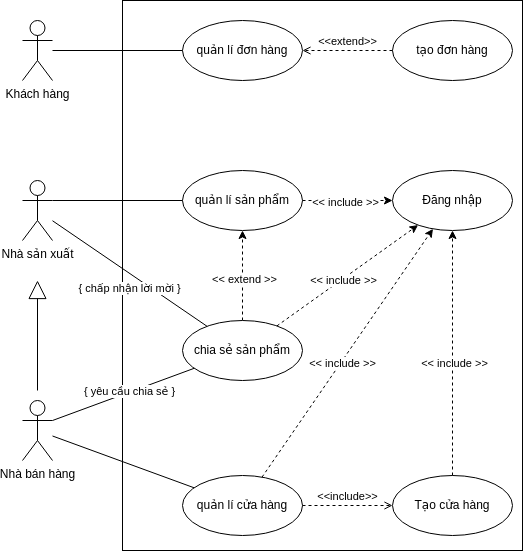
\includegraphics[width=0.8\textwidth]{usecase-usecase}
	\caption{Sơ đồ ca sử dụng tổng quát}
	\justifying
	Khách hàng có thể đặt hàng và xem đơn hàng vừa đặt mà không cần đăng nhập. Nhà sản xuất có thể mở tài khoản để đăng tải thông tin về doanh nghiệp cũng như sản phẩm của mình. Sau đó chia sẻ cho các nhà bán hàng để phân phối thông tin này đến các nhà bán hàng.
\end{figure}
\clearpage
\subsubsection{Tính năng đăng nhập}
\begin{figure}[hbt!]\fontsize{13px}{13px}\selectfont
\centering
		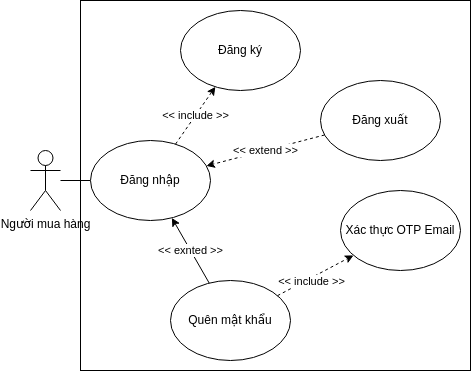
\includegraphics[width=0.7\textwidth]{usecase-login}
		\caption{Sơ đồ ca đăng nhập}
\justifying
Chức năng đăng nhập bao gồm tính năng đăng ký. Trong trường hợp quên mật khẩu, người dùng có thể xác thực đặt lại thông tin mật khẩu thông qua hộp thư điện tử.
\end{figure}

\subsubsection{Tính năng quản lí sản phẩm}
\begin{figure}[hbt!]\fontsize{13px}{13px}\selectfont
\centering
		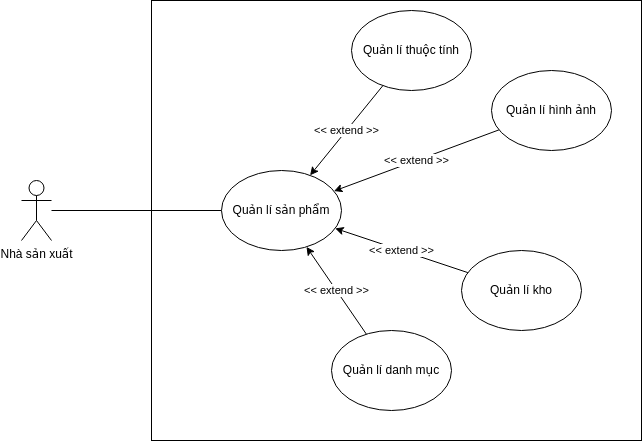
\includegraphics[width=0.6\textwidth]{usecase-sellers}
		\caption{Sơ đồ ca quản lí sản phẩm}
\justifying
Quản lí sản phẩm bao gồm tất cả các tính năng liên quan phục vụ cho việc đăng tải thông tin sản phẩm. Bao gồm thông tin tồn kho của sản phẩm đó.
\end{figure}

\subsubsection{Tính năng chia sẻ sản phẩm}
\begin{figure}[hbt!]\fontsize{13px}{13px}\selectfont
\centering
		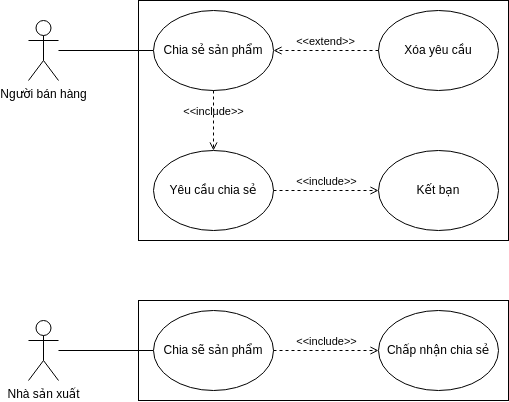
\includegraphics[width=0.6\textwidth]{usecase-contract}
		\caption{Sơ đồ ca yêu cầu chia sẻ}
\justifying
Tính năng chia sẻ sản phẩm giúp cho nhà sản xuất đăng tải, phân phối thông tin của họ trên các trang của nhà bán hàng. Tính năng này yêu cầu sử dụng tính năng kết bạn trước đó.
\end{figure}

\subsubsection{Tính năng kết bạn}
\begin{figure}[hbt!]\fontsize{13px}{13px}\selectfont
\centering
		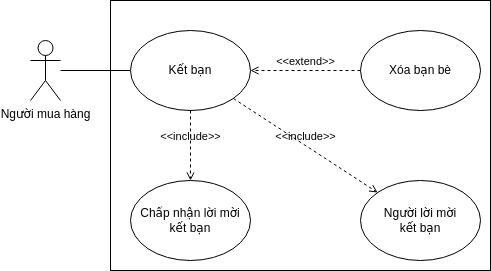
\includegraphics[width=0.6\textwidth]{usecase-relationship}
		\caption{Sơ đồ ca trường hợp kết bạn}
\justifying
Tính năng kết bạn yêu cầu người dùng phải biết username của nhau trước đó. Thông qua username, giữa hai người có thể gửi lời mời kết bạn cho nhau hoặc xác nhận.
\end{figure}

\clearpage
\subsubsection{Tính năng quản lí cửa hàng}
\begin{figure}[hbt!]\fontsize{13px}{13px}\selectfont
\centering
		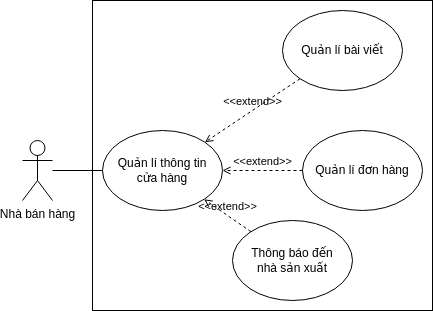
\includegraphics[width=0.5\textwidth]{usecase-store}
		\caption{Sơ đồ ca trường hợp quản lí cửa hàng}
\justifying
Với tính năng quản lí cửa hàng, nhà bán hàng có thể chỉnh sửa thông tin của cửa hàng. Ví dụ như cài đặt màu thương hiệu, tên cửa hàng, slogan, mã số doanh nghiệp,... Các đơn hàng được đặt trên trang sẽ thuộc về người nhà bán hàng.
\end{figure}

\subsubsection{Tính năng đặt hàng}
\begin{figure}[hbt!]\fontsize{13px}{13px}\selectfont
\centering
		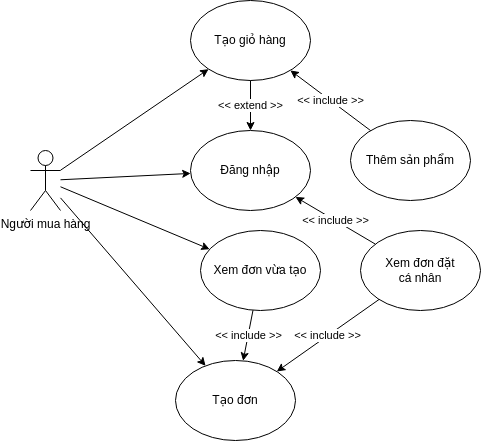
\includegraphics[width=0.7\textwidth]{usecase-order}
		\caption{Sơ đồ ca đặt hàng}
\justifying
Tính năng đặt hàng giúp người mua hàng để lại thông tin mua hàng bao gồm địa chỉ nhận hàng và thông tin số lượng thuộc tính của từng sản phẩm đặt mua. Sử dụng tính năng đặt hàng cũng đồng thời gửi thông báo đến người sở hữu cửa hàng về thông tin đơn hàng.
\end{figure}

% Tính năng chia sẻ là khi lời mời được chấp nhận, sản phẩm của trang thương mại điện tử này có thể hiển thị và đặt mua ở trên trang khác. Nếu có cập nhật thì sản phẩm sẽ tự động đồng bộ.

\clearpage
\subsubsection{Tính năng thông báo}
\begin{figure}[hbt!]\fontsize{13px}{13px}\selectfont
\centering
		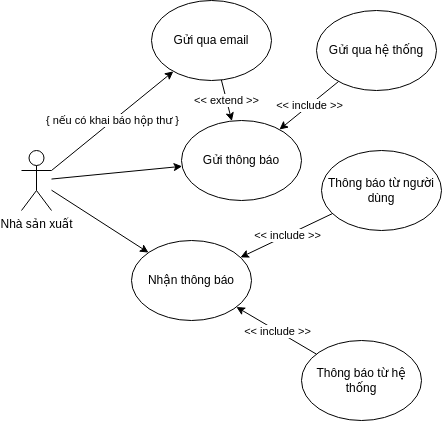
\includegraphics[width=0.8\textwidth]{usecase-notification}
		\caption{Sơ đồ ca trường hợp thông báo}
\justifying
Tính năng thông báo giúp nhà bán hàng gửi thông báo cho nhà sản xuất hoặc ngược lại. Đồng thời, thông qua tính năng này. Hệ thống có thể gửi thông báo đơn hàng đến nhà bán hàng khi có đơn hàng được tạo.

Thông báo chia làm hai loại là thông báo hệ thống và thông báo thư điện tử. Thông báo hệ thống sẽ gửi đến giao diện hệ thống của người nhận. Thông báo thư điện tử sẽ thực hiện chức năng giống hệt như hành động gửi thư điện tử thông thường nhưng khác ở chỗ các thông tin thư sẽ được lưu trữ và hiển thị một phần trên giao diện của hệ thống.
\end{figure}